\pdfoutput=1
\documentclass[11pt]{article}

\PassOptionsToPackage{numbers,compress}{natbib}
\usepackage[preprint]{neurips_2026}

\usepackage[T1]{fontenc}
\usepackage[utf8]{inputenc}
\usepackage{microtype}
\usepackage{amsmath}
\usepackage{amssymb}
\usepackage{booktabs}
\usepackage{tabularx}
\usepackage{array}
\usepackage{enumitem}
\usepackage{xcolor}
\usepackage{graphicx}
\usepackage{tikz}
\usepackage{hyperref}
\usepackage{url}
\usepackage{listings}

\usetikzlibrary{arrows.meta,positioning,fit,shapes.geometric}

\hypersetup{
  colorlinks=true,
  linkcolor=blue!50!black,
  citecolor=blue!50!black,
  urlcolor=blue!50!black
}

\lstdefinestyle{pncode}{
  basicstyle=\ttfamily\small,
  frame=single,
  breaklines=true,
  columns=fullflexible,
  keepspaces=true,
  backgroundcolor=\color{gray!4}
}

\newcommand{\papernexus}{\textsc{PaperNexus}}
\newcommand{\mcp}{\textsc{MCP}}
\newcommand{\code}[1]{\texttt{\detokenize{#1}}}
\newcolumntype{Y}{>{\raggedright\arraybackslash}X}

\title{\papernexus: A Local-First Research Harness for Paper-Centered Knowledge Work}

\author{
  PaperNexus Project
}

\date{}

\begin{document}

\maketitle

\begin{abstract}
\papernexus{} is a local-first research harness for paper-centered knowledge work. It helps a researcher move from a topic or corpus to an inspectable research memory: literature candidates, legal full-text availability, parsed paper snapshots, typed knowledge-graph entities, method-evolution evidence, cross-domain research answers, retrieval benchmarks, and operational views for humans and agents. The central failure mode addressed by the system is unsupported plausibility: a research assistant may produce a convincing synthesis while losing track of which papers, claims, methods, quotes, access decisions, and evaluation outcomes justify that synthesis.

This report presents \papernexus{} as a functional system rather than a code artifact. As of May 10, 2026, the system has seven user-facing layers. The discovery layer turns a topic into merged paper candidates and explicit open-access status. The ingestion layer converts local PDFs or Markdown files into reusable semantic snapshots. The graph layer stores papers, problems, methods, claims, evidence, datasets, benchmarks, ideas, and method-to-method relationships. The intelligence layer answers questions through graph evidence, method lineage, cross-domain mechanism search, and idea-catalyst workflows. The evaluation layer measures retrieval and task behavior against BEIR-style, biomedical, literature-search, and custom benchmarks. The security layer supports encrypted local environment variables and sanitized release artifacts. The interface layer exposes the same research memory through a command-line interface, browser dashboard, authenticated HTTP APIs, local stdio \mcp{}, remote streamable HTTP \mcp{}, and Python helper scripts. The result is a research environment designed to preserve evidence, support staged reuse, and make long-running literature work auditable.
\end{abstract}

\section{Introduction}

Academic research increasingly depends on long chains of machine assistance: search engines retrieve candidate papers, PDF parsers extract text, language models summarize sections, graph tools connect ideas, and agents turn intermediate notes into research plans. The practical bottleneck is no longer only whether a system can find a paper. It is whether the system can preserve enough structure for a later user to ask: Where did this claim come from? Which method improved which predecessor? Was the cited paper actually available as an open PDF? Which part of the corpus supports this cross-domain analogy?

\papernexus{} is built around a conservative assumption:

\begin{quote}
If research memory is represented only as files, embeddings, or prompt-time summaries, then evidence can become detached from the claims that depend on it.
\end{quote}

The system therefore treats the research graph as the primary artifact. Papers are not only documents to retrieve; they are sources of typed objects such as problems, methods, claims, evidence, datasets, benchmarks, takeaways, idea fragments, and future directions. Literature discovery is not only a download helper; it is a record of what was searched, merged, resolved, skipped, and legally available. Research answers are not only generated prose; they are views over an evidence-bearing graph.

This paper follows the style of functional technical reports for research harnesses such as ARIS~\citep{yang2026aris}: it emphasizes the operating assumptions, architectural layers, workflow surfaces, assurance mechanisms, evaluation hooks, and deployment footprint of the system. We intentionally de-emphasize line-by-line implementation details. The goal is to explain what a researcher can do with \papernexus{}, how the pieces fit together, and why the system is organized around local ownership, explicit evidence, and measurable behavior.

\section{Functional Thesis}

The system is designed around three claims.

\paragraph{Research work needs durable memory.}
A literature review does not end when a set of snippets is retrieved. The researcher needs to revisit earlier parses, compare method families, inspect unresolved sources, and ask new questions without repeating the whole pipeline. \papernexus{} therefore stores raw sources, markdown cache, semantic snapshots, graph artifacts, queue state, discovery outputs, and derived overlays as local, reusable assets.

\paragraph{Evidence should be represented before answers are generated.}
For paper-centered work, the most useful automation surface is often not a chatbot response but a structured memory that can later support many responses. \papernexus{} places graph construction before answer construction. Question answering, method lineage, cross-domain search, and idea generation operate over committed graph state rather than relying on query-time invention.

\paragraph{Automation must remain inspectable.}
The system exposes its state through multiple surfaces: CLI commands for operators, a browser dashboard for inspection, HTTP APIs for applications, \mcp{} tools for agents, and Python scripts for remote workflows. These interfaces are different views of the same local research memory rather than independent silos.

\paragraph{Evaluation and secrets must be first-class operational concerns.}
A research harness that discovers papers, calls external providers, and serves remote agents must be evaluated and sanitized before it is shared. \papernexus{} therefore includes retrieval-benchmark loaders and metrics, encrypted local environment storage, bearer-token guarded server surfaces, and a release-hygiene path that removes personal paths, accounts, local state, and generated build traces from public artifacts.

\section{System Overview}

Figure~\ref{fig:functional} summarizes the functional architecture. The left side introduces sources, the center maintains durable research memory, and the right side exposes human and agent workflows.

\begin{figure}[t]
\centering
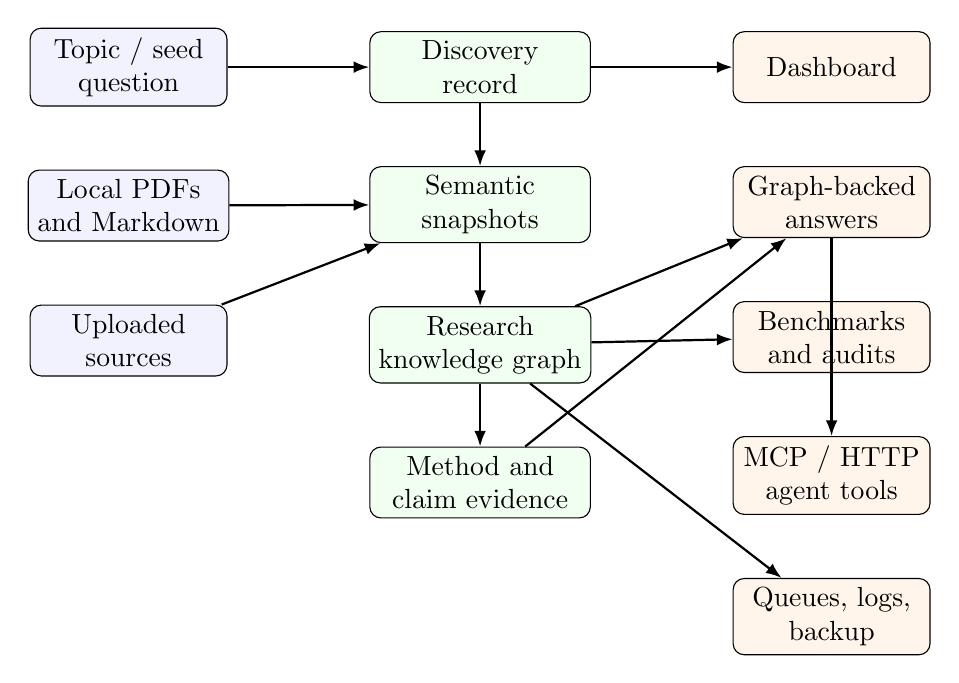
\begin{tikzpicture}[
  node distance=8mm and 9mm,
  block/.style={draw, rounded corners, align=center, minimum width=25mm, minimum height=9mm, fill=blue!5},
  mem/.style={draw, rounded corners, align=center, minimum width=28mm, minimum height=9mm, fill=green!6},
  iface/.style={draw, rounded corners, align=center, minimum width=25mm, minimum height=9mm, fill=orange!8},
  arrow/.style={-{Latex[length=2mm]}, thick}
]
  \node[block] (topic) {Topic / seed\\question};
  \node[block, below=of topic] (files) {Local PDFs\\and Markdown};
  \node[block, below=of files] (imports) {Uploaded\\sources};

  \node[mem, right=18mm of topic] (discovery) {Discovery\\record};
  \node[mem, below=of discovery] (snapshots) {Semantic\\snapshots};
  \node[mem, below=of snapshots] (graph) {Research\\knowledge graph};
  \node[mem, below=of graph] (evidence) {Method and\\claim evidence};

  \node[iface, right=18mm of discovery] (dashboard) {Dashboard};
  \node[iface, below=of dashboard] (answers) {Graph-backed\\answers};
  \node[iface, below=of answers] (eval) {Benchmarks\\and audits};
  \node[iface, below=of eval] (agents) {MCP / HTTP\\agent tools};
  \node[iface, below=of agents] (ops) {Queues, logs,\\backup};

  \draw[arrow] (topic) -- (discovery);
  \draw[arrow] (files) -- (snapshots);
  \draw[arrow] (imports) -- (snapshots);
  \draw[arrow] (discovery) -- (snapshots);
  \draw[arrow] (snapshots) -- (graph);
  \draw[arrow] (graph) -- (evidence);
  \draw[arrow] (discovery) -- (dashboard);
  \draw[arrow] (graph) -- (answers);
  \draw[arrow] (evidence) -- (answers);
  \draw[arrow] (graph) -- (eval);
  \draw[arrow] (answers) -- (agents);
  \draw[arrow] (graph) -- (ops);
\end{tikzpicture}
\caption{Functional view of \papernexus{}. Discovery, ingestion, graph memory, evidence, benchmark, agent, and operations layers are maintained as local artifacts or controlled interfaces without changing the local ownership model.}
\label{fig:functional}
\end{figure}

\subsection{Layered Responsibilities}

\begin{table}[t]
\centering
\caption{Functional layers in \papernexus{}.}
\label{tab:layers}
\begin{tabularx}{\linewidth}{@{}lY@{}}
\toprule
Layer & Role in the research workflow \\
\midrule
Discovery & Turns a topic into provider queries, merged candidates, open-access status, download manifests, and importable sources. \\
Ingestion & Converts local PDFs or Markdown into reusable paper snapshots with parser metadata and semantic extraction results. \\
Graph memory & Represents papers, problems, methods, claims, evidence, datasets, benchmarks, takeaways, ideas, and relations as a persistent local graph. \\
Evidence & Tracks method evolution, citation contexts, exact quotes, temporal direction, confidence, and blocked or ambiguous relationships. \\
Interfaces & Provides CLI, Web UI, HTTP API, local \mcp{}, remote HTTP \mcp{}, services, logs, and Python wrappers. \\
Evaluation and hygiene & Measures retrieval and task behavior, stores encrypted local secrets, and sanitizes release artifacts before publication. \\
\bottomrule
\end{tabularx}
\end{table}

The separation is practical. Discovery can be repeated without rebuilding the graph. Parsing can be retried without losing the source manifest. Graph construction can be staged and committed after inspection. Interfaces can query committed state without re-running expensive upstream work.

\section{Functional Workflows}

\subsection{Topic to Corpus}

The discovery workflow starts from a topic, seed question, related-work paragraph, venue, author, dataset, or manually supplied paper. It plans complementary queries, sends them to open metadata providers, merges candidates, expands through citations when available, and resolves legal full-text sources. It uses services such as OpenAlex~\citep{openalex}, Semantic Scholar~\citep{semanticscholar}, Crossref~\citep{crossref}, arXiv~\citep{arxivapi}, DBLP~\citep{dblp}, Europe PMC~\citep{europepmc}, CORE~\citep{coreapi}, and Unpaywall~\citep{unpaywall}.

The important output is not merely a folder of PDFs. The workflow records what was found and why a candidate could or could not enter the corpus. A result may be a resolved open PDF, a metadata-only paper, an item requiring institutional access, an access-control-blocked page, or a URL that returned HTML instead of a PDF. This distinction matters because a research assistant should not confuse ``not downloaded'' with ``not relevant'' or with ``not legally available.'' The current implementation persists discovery runs with JSON artifacts, Markdown reports, download manifests, import-task links, candidate provenance, and latest-run pointers.

\subsection{Corpus to Research Memory}

Once sources exist locally, \papernexus{} materializes them into reusable semantic snapshots. The default path parses PDF or Markdown, stores markdown cache and metadata, and allows later LLM-assisted enrichment to run as a separate stage. This gives the user a durable intermediate representation: if graph construction changes, the system can reuse prior parsing rather than starting from raw PDFs.

The staged pipeline is intentionally simple:

\begin{lstlisting}[style=pncode]
sources -> materialize -> llm-optimize -> build-graph
        -> merge-graph -> write-index
\end{lstlisting}

The key property is resumability. A user can run the full analysis once, continue after interruption, rebuild only dirty stages, or inspect stage outputs before committing a new graph.

\subsection{Research Memory to Evidence}

The graph layer makes paper-centered objects queryable. Problems, methods, claims, evidence, datasets, benchmarks, takeaways, idea fragments, and future directions become typed nodes. Relations between them become explicit edges. This enables both conventional literature exploration and higher-level reasoning tasks.

Method evolution is treated as a special evidence problem. A system should not casually claim that one method extends, improves, replaces, adapts, or uses another method. \papernexus{} therefore records method aliases, citation contexts, quote evidence, candidate relationships, accepted relationships, stubs, and diagnostics. Strong method-evolution relationships require support beyond name overlap: the relationship must be grounded in context, direction, and confidence.

\subsection{Evidence to Answers}

Research-intelligence workflows read from graph state. They can answer cross-domain questions, produce method lineages, inspect evidence for a method relationship, return a method registry, or combine these views into a unified answer. The operating invariant is that these workflows should expose existing graph evidence rather than silently generate new evidence at query time.

This gives the system a useful division of labor. Language models may help enrich snapshots or phrase responses, but the evidence substrate remains an inspectable local graph. When a researcher asks for a mechanism, lineage, or analogy, the answer can point back to the corpus state that supports it.

\subsection{Research Memory to Evaluation}

\papernexus{} now includes a retrieval-benchmark path that can evaluate the discovery and retrieval surface rather than only describe it qualitatively. The benchmark command supports closed-corpus and live-discovery modes. Closed-corpus mode follows information-retrieval semantics: the system searches a provided corpus and is scored against query relevance labels. Live mode runs the normal provider-backed discovery workflow and scores returned papers against gold identifiers or titles.

The loader surface covers custom JSON/JSONL, BEIR-style corpora and TREC qrels, LitSearch-style query/corpus exports, BioASQ question files, native TREC biomedical topics plus qrels, CSFCube faceted annotations, and flexible schemas for SAGE, ScholarQABench/OpenScholar, PaperAsk, SPARBench, and SciNetBench. The reported metrics include hit@k, exact match@k, recall@k, weighted recall@k, precision@k, F1@k, MRR@k, MAP@k, and NDCG@k. For task-style benchmarks, \papernexus{} can additionally score answer overlap, citation precision and recall, claim-label accuracy, relation/path overlap, and optional LLM-judged answer grounding.

\section{Interface Surface}

\papernexus{} exposes the same research memory through several interfaces (Table~\ref{tab:interfaces}). This is a functional choice rather than a convenience layer: different users need different levels of control over the same corpus.

\begin{table}[t]
\centering
\caption{Interface surfaces and their intended users.}
\label{tab:interfaces}
\begin{tabularx}{\linewidth}{@{}lY@{}}
\toprule
Interface & Typical use \\
\midrule
CLI & Initialize a corpus, run staged analysis, inspect status, search the graph, benchmark retrieval, manage secure environment values, export backups, and manage services. \\
Dashboard & Inspect corpus status, graph summaries, overlays, imports, runtime configuration, and human-readable views. \\
HTTP API & Integrate browser and server workflows with authenticated routes for graph, method-evidence, discovery, and research-answer queries. \\
Local \mcp{} & Give a local coding or research agent tool access over stdio. \\
Remote HTTP \mcp{} & Expose the same agent tool surface from a running server with bearer-token authentication. \\
Python wrappers & Submit imports, inspect queues, query graph state, and orchestrate remote workflows from scripts. \\
Secure environment & Keep local provider keys and runtime secrets in an encrypted file whose encryption key is held by the system keychain. \\
\bottomrule
\end{tabularx}
\end{table}

The \mcp{} surface follows the Model Context Protocol~\citep{mcp}. Its purpose is to make research memory available to agents without asking those agents to understand the internal storage layout. Important tool families include literature discovery, research lookup, research briefing, idea catalyst, and import workflow.

\section{Assurance Mechanisms}

\papernexus{} does not claim that every extracted relationship is correct. Instead, it makes uncertainty and evidence boundaries visible.

\paragraph{Access assurance.}
Discovery records whether full text is open, unavailable, restricted, blocked, or malformed. This prevents downstream tools from treating access failure as absence of evidence.

\paragraph{Snapshot assurance.}
Parsing and semantic extraction are separated from graph commit. A failed parser, degenerate title, or incomplete snapshot can be detected before it pollutes the graph.

\paragraph{Graph assurance.}
The graph schema constrains the kinds of objects and relationships that can be represented. Lite projections and metadata make committed state inspectable without requiring the full graph engine for every read.

\paragraph{Method-evidence assurance.}
Strong method-evolution edges require resolved methods, citation context, quote support, confidence, temporal direction, and non-conflicting evidence. Ambiguous aliases and stubs are preserved as diagnostics rather than silently promoted.

\paragraph{Operational assurance.}
Queues, logs, backups, and staged commands allow the user to recover from interruptions and audit long-running work. This is especially important when imports, PDF parsing, and LLM enrichment run over large corpora.

\paragraph{Evaluation assurance.}
Retrieval benchmarks separate fixed-corpus scores from live-provider scores. This prevents a live API run from being mistaken for an official leaderboard run and makes provider availability, source resolution, and corpus retrieval quality visible as distinct measurements.

\paragraph{Credential and release assurance.}
Local credentials can be loaded from encrypted secure-env storage, and public release artifacts can be sanitized so that personal account names, absolute home paths, local caches, bearer-token fixtures, and LaTeX build traces do not leak into documentation or arXiv source bundles.

\section{Functional Footprint}

Table~\ref{tab:footprint} summarizes the current feature footprint without tying the description to source files.

\begin{table}[t]
\centering
\caption{Current functional footprint.}
\label{tab:footprint}
\begin{tabularx}{\linewidth}{@{}lY@{}}
\toprule
Function & Current behavior \\
\midrule
Literature discovery & Plans queries, merges multi-provider candidates, resolves legal full text, records coverage, and bridges resolved sources into the import queue. \\
PDF and Markdown ingestion & Supports local corpora and uploaded import tasks with parser configuration, fallback parsing, markdown cache, and semantic snapshots. \\
Graph construction & Builds a typed research graph and commits a lightweight read projection for query, dashboard, and agent workflows. \\
Method evolution & Builds method registries, validates method-to-method evidence, records candidates and accepted relationships, and exposes lineage/evidence lookups. \\
Research answers & Provides graph-backed cross-domain evidence, method lineage, method evidence, method registry, and unified answer modes. \\
Retrieval evaluation & Runs fixed-corpus and live-discovery retrieval benchmarks over custom, BEIR-style, biomedical, literature-search, and graph-reasoning benchmark formats. \\
Security hygiene & Provides encrypted local secure-env storage, bearer-token authenticated server surfaces, portable path helpers, and sanitized release artifacts. \\
Operations & Supports services, logs, dashboard serving, authenticated remote \mcp{}, backup export, backup unpack, and queue inspection. \\
\bottomrule
\end{tabularx}
\end{table}

\section{Example Use Patterns}

\paragraph{Literature mapping.}
A researcher starts with a topic such as ``graph-augmented experiment planning.'' \papernexus{} searches open metadata providers, merges duplicate candidates, records which papers have legal full-text access, imports resolved PDFs, and builds a graph that supports later search over problems, methods, claims, evidence, and datasets.

\paragraph{Method lineage review.}
A researcher asks how a method family evolved. The system looks for validated method-to-method relationships, reports predecessor and successor links, and exposes the citation contexts and quote evidence that support the relationship. The user can distinguish a substantive improvement claim from a mere background comparison.

\paragraph{Cross-domain ideation.}
A researcher looks for mechanisms from one domain that might transfer to another. \papernexus{} uses domain bridge, analogy, catalyst, and graph-evidence workflows to propose candidates grounded in the existing corpus rather than free-form brainstorming alone.

\paragraph{Agent-assisted research.}
A coding or research agent connects to local or remote \mcp{}. Instead of scraping folders directly, the agent can call tools for discovery status, graph lookup, research answers, paper index lookup, import workflow, and idea-catalyst operations.

\paragraph{Retrieval benchmarking.}
A researcher evaluates whether a discovery strategy is actually returning expected papers. In fixed-corpus mode, \papernexus{} reads a benchmark corpus, query set, and qrels, then reports ranking metrics. In live mode, the same benchmark query can exercise OpenAlex, Semantic Scholar, Crossref, arXiv, and configured optional providers. This makes external-provider behavior measurable without conflating it with closed-corpus retrieval quality.

\section{Deployment Observations}

The current implementation is a functional research harness with an implemented benchmark entry point, but not yet a published benchmark result suite. The observed system state supports four practical conclusions.

First, the architecture is coherent: discovery feeds ingestion, ingestion feeds graph construction, method evidence attaches to graph memory, and intelligence workflows consume committed graph state. Second, the interface strategy is useful: the same local research memory can be operated from CLI, dashboard, HTTP, \mcp{}, and scripts. Third, the evaluation surface is now concrete enough to support fixed-corpus and live-discovery retrieval experiments before a public benchmark table is reported. Fourth, release maturity should be judged through functional smoke tests, security scans, and unit tests: discovery should be exercised on small topics, method lineage should be queried through remote \mcp{}, parser/runtime configuration should be checked on the target machine, and release artifacts should be scanned for private paths or credentials before distribution.

For this May 10 report build, local verification included the full Node test suite and a release-hygiene scan. The test suite passed 366 of 366 tests. The scan found no repository-text, arXiv-source, or PDF string matches for private home paths, personal account names, long bearer-token literals, OpenAI-style keys, GitHub-style tokens, or private-key blocks.

\section{Limitations and Future Work}

\papernexus{} has several current limitations.

First, metadata-only discovery candidates are recorded but are not automatically promoted into full graph paper nodes unless they pass through import and materialization. Second, discovery source coverage remains incomplete: OpenReview, Papers with Code, DataCite, OpenAIRE, BASE, HAL, Zenodo, bioRxiv, medRxiv, SSRN, OSF, and Chinese scholarship providers are natural extensions. Third, systematic-review-style screening is not yet a standalone workflow with include/exclude tables and reviewer decisions. Fourth, version relations such as preprint-of, extended-by, artifact-for, and dataset-for are not yet fully represented as graph relations. Fifth, the benchmark layer has loaders and metrics but still needs reported runs on public and private gold sets. Sixth, method-evolution quality depends on extraction quality; conservative validation reduces false positives but may miss valid but weakly expressed relationships.

Future evaluation should therefore focus on functional outcomes: discovery recall against systematic-review gold sets, open-access status accuracy, parser success and metadata accuracy, graph entity and relation precision, method-edge precision, fixed-corpus retrieval quality, live-provider retrieval quality, and answer faithfulness. These measurements should complement engineering checks such as latency, throughput, queue recovery, service stability, and secure release hygiene.

\section{Conclusion}

\papernexus{} is a local-first research harness for turning paper-centered work into durable, inspectable research memory. Its main contribution is not a single retrieval model or a single agent prompt. It is the integration of discovery, ingestion, graph construction, method-evidence validation, graph-backed research intelligence, and multi-surface operation into one local workflow.

The system is designed for researchers who want automation without giving up provenance. It records what was searched, what was resolved, what was parsed, what entered the graph, what evidence supports a relationship, and what interface exposed the result. In that sense, \papernexus{} treats research assistance as a memory and evidence problem first, and a generation problem second.

\section*{Acknowledgments}

This report was generated from the local \papernexus{} working tree and project documentation on May 10, 2026. The writing style was revised to follow the functional technical-report pattern exemplified by ARIS~\citep{yang2026aris}; no text from that paper is reused.

\bibliographystyle{plainnat}
\bibliography{references}

\appendix

\section{Functional Command Sketch}

The most common operator path is:

\begin{lstlisting}[style=pncode]
papernexus init
papernexus analyze --force
papernexus serve
\end{lstlisting}

The staged path exposes intermediate state:

\begin{lstlisting}[style=pncode]
papernexus materialize --continue
papernexus llm-optimize --continue
papernexus build-graph --continue
papernexus merge-graph --continue
papernexus write-index --continue
\end{lstlisting}

Retrieval evaluation can be run in fixed-corpus mode:

\begin{lstlisting}[style=pncode]
papernexus benchmark-retrieval ./benchmarks/scifact \
  --format beir \
  --evaluation-mode fixed-corpus \
  --k 1,5,10,20
\end{lstlisting}

Local secrets can be stored outside plain configuration files:

\begin{lstlisting}[style=pncode]
papernexus secure-env set OPENAI_API_KEY
papernexus secure-env list
\end{lstlisting}

\section{Remote Agent Pattern}

Remote agent access is enabled by running the dashboard server with authenticated streamable HTTP \mcp{}. A client can then call graph lookup, literature discovery, import workflow, and idea-catalyst tools against the same corpus that the local dashboard displays. This pattern is useful when the research corpus stays on one machine but agents or scripts run from another environment.

\end{document}
